\documentclass{beamer}
\usepackage[croatian]{babel}
\usepackage[utf8]{inputenc}
\usepackage{tikz}
\usepackage{float}
\usepackage{graphicx}
\usepackage{booktabs}
\usepackage{color}

% Informacije za naslovnicu
\title{Nadopunjavanje slike korištenjem difuzijskih modela}
\author{Martin Bakač, Mislav Đomlija, Ivan Kapusta, Maksim Kos, Antonio Lukić, Jerko Šegvić}
\institute{Sveučilište u Zagrebu, Fakultet elektrotehnike i računarstva}
\date{2025}
\titlegraphic{
\includegraphics[width=2.5cm]{images/FER_logo.png}} 

\begin{document}

% Naslovna stranica
\frame{\titlepage}

% Uvod
\begin{frame}
    \frametitle{Nadopunjavanje slike}
    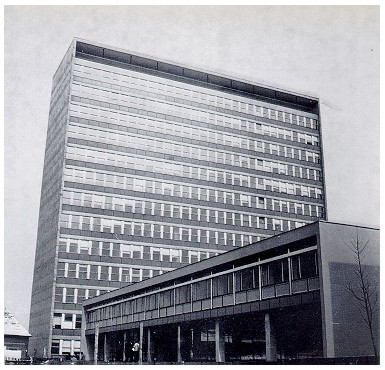
\includegraphics[width=5cm]{images/fer1.jpg}
    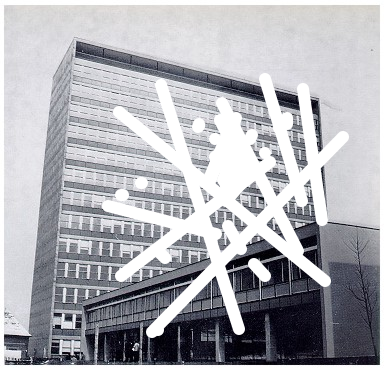
\includegraphics[width=5cm]{images/fer2.png}
\end{frame}

\begin{frame}
    \frametitle{Nadopunjavanje slike}
    \begin{itemize}
        \item Nadopunjavanje slike (engl. \emph{image inpainting}) zamjenjuje nedostajuće piksele slike uvjerljivim sadržajem.
        \pause
        \item Modeli za nadopunu slike zahtijevaju snažne generativne sposobnosti.
        \pause
        \item Popularni pristupi: generativne suparničke mreže (GAN), autoregresivni modeli, difuzijski modeli.
    \end{itemize}
\end{frame}

% Difuzijski modeli
\begin{frame}
    \frametitle{Difuzijski modeli}
    \begin{itemize}
        \item Difuzijski modeli simuliraju reverznu difuziju za generiranje podataka iz latentnog prostora.
        \pause
        \item Dva ključna procesa:
        \begin{itemize}
            \item \textbf{Unaprijedni proces:} Dodavanje šuma podacima.
            \item \textbf{Reverzni proces:} Uklanjanje šuma za rekonstrukciju.
        \end{itemize}
    \end{itemize}
\end{frame}

% UNet arhitektura
\begin{frame}
    \frametitle{UNet arhitektura}
    \begin{itemize}
        UNet mreža za učenje unazadnog koraka difuzije.
    \end{itemize}
    \center
    \begin{figure}
        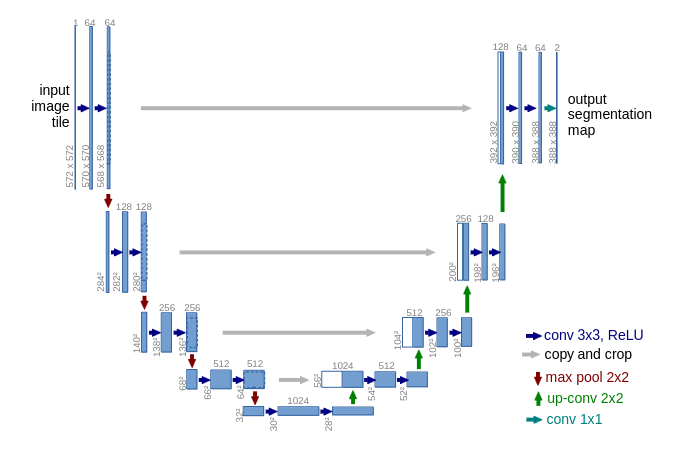
\includegraphics[width=0.8\textwidth]{images/unet.png}
        \caption{Ronneberger et al.2015}
    \end{figure}
\end{frame}

% RePaint algoritam
\begin{frame}
    \frametitle{RePaint algoritam}
    \begin{itemize}
        \item Algoritam za nadopunjavanje slike korištenjem difuzijskih modela.
        \pause
        \item Kombinira vidljive dijelove slike s generiranima u reverznom procesu.
    \end{itemize}
    \pause
    \center
    \begin{figure}
        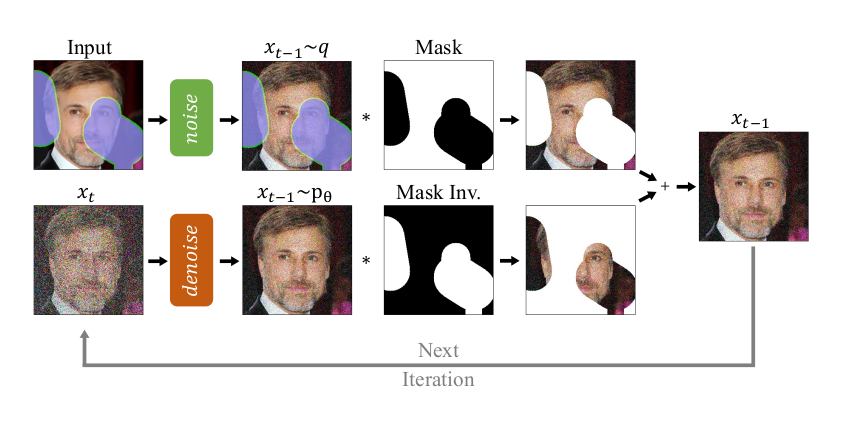
\includegraphics[width=0.8\textwidth]{images/repaint.png}
        \caption{Lugmayr et al.2022}
    \end{figure}
\end{frame}

% Rezultati
\begin{frame}
    \frametitle{Rezultati nadopunjavanja}
    \begin{itemize}
        \item Model treniran na MNIST-u.
        \pause
        \item Uspješno popunjavanje složenih praznina.
        \pause
    \end{itemize}
    
\includegraphics[width=0.45\textwidth]{../repaint_output/inpainted_combined_6.png}
    
\includegraphics[width=0.45\textwidth]{../repaint_output/inpainted_combined_7.png}
    
\includegraphics[width=0.45\textwidth]{../repaint_output/inpainted_combined_4.png}
    
\includegraphics[width=0.45\textwidth]{../repaint_output/inpainted_combined_1.png}
\end{frame}

% Zaključak
\begin{frame}
    \frametitle{Zaključak}
    \begin{itemize}
        \item Difuzijski modeli pokazali su robusnost u nadopunjavanju slika.
        \pause
        \item Prednosti:
        \begin{itemize}
            \item Fleksibilnost maskiranja.
            \item Korištenje predtreniranih modela.
            \item Generiranje uvjerljivih rezultata.
        \end{itemize}
        \pause
        \item Izazovi u optimizaciji brzine i kvalitete generiranja.
    \end{itemize}
\end{frame}

\begin{frame}{}
  \centering \Large
  \emph{Hvala na pažnji.}
\end{frame}

\end{document}
